\chapter{Implementation}
\label{cha:Implementation}
The final implementation was done in Java, an was built on top of the AIM simulator codebase. All class diagrams were created using IntelliJ IDEA 15.0.3 internal diagram tool. Figure \ref{fig:classDiagramKey} provides a key for understanding these diagrams.

\section{Generalising the Codebase}
\label{sec:Generalising the Codebase}
\begin{tabular}{|c|c|c|}
\hline
Requirement Code & Acheived? \\
\hline
NS.11 & \cellcolor{green} \checkmark \\
NS.12 & \cellcolor{green} \checkmark \\
\hline
\end{tabular}

The use of the AIM codebase was a project restriction imposed for research purposes. By working with the AIM simulator codebase I could learn how easy it is to work with, and analyse whether or not it will be a good codebase to continue expanding upon for future AV projects. Each simulator built for this project works alongside the AIM simulators, whilst being completely independent. The project: 'A self-organising approach to autonomous vehicle car park management using a message-based protocol' \citep{Milligan2017}, also uses simulators built using AIM. To make sure that code coupling was reduced as much as possible, I worked closely with their project lead to generalise the codebase, breaking out useful shared features so that they could be accessed by all simulator types.

\begin{figure}[htb]
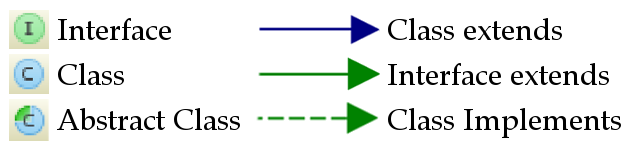
\includegraphics[width=\textwidth]{classDiagrams/classDiagramKey.png}
\caption{Key for the class diagrams in this report.}
\label{fig:classDiagramKey}
\end{figure}

\todo{Decide what to put here} Appendix \ref{sec:Generalising the Codebase Appendix} provides detailed coverage of both this change, and changes made to some of the other areas of the AIM codebase.

\section{GUI}
\label{sec:GUI}
\begin{tabular}{|c|c|c|}
\hline
Requirement Code & Acheived? \\
\hline
FS.11 & \cellcolor{green} \cmark \\
FS.21 & \cellcolor{green} \cmark \\
FS.31 & \cellcolor{green} \cmark \\
FS.41 & \cellcolor{green} \cmark \\
FS.51 & \cellcolor{green} \cmark \\
FS.61 & \cellcolor{green} \cmark \\
FS.72 & \cellcolor{green} \cmark \\
FS.82 & \cellcolor{red} \xmark \\
FS.92 & \cellcolor{red} \xmark \\
FS.101 & \cellcolor{green} \cmark \\
FS.111 & \cellcolor{green} \cmark \\
FS.121 & \cellcolor{green} \cmark \\
FS.131 & \cellcolor{green} \cmark \\
FS.141 & \cellcolor{green} \cmark \\
FS.151 & \cellcolor{green} \cmark \\
FS.161 & \cellcolor{green} \cmark \\
FS.171 & \cellcolor{red} \xmark \\
\hline
\end{tabular}

The GUI for the project was built using 

\section{Map}
\label{sec:Map}

\section{Simulation}
\label{sec:Simulation}

\section{Merge Schemes}
\label{sec:Merge Schemes}

\section{Results Production}
\label{sec:Results Production}

\section{Testing}
\label{sec:Testing}

\subsection{Unit Testing}
\label{subsec:Unit Testing}
Unit tests were mostly used to ensure getter and setter methods worked as expected. However, some unit tests were used to verify the behaviour of classes. To do this I used Mockito \citep{MockitoWebsite} to mock the behaviour of objects used by the test class so that I could prompt the test class into producing the expected results.

\subsection{Integration Tests}
\label{subsec:Integration Tests}

